\documentclass{article}

%\usepackage{codespace}

% Encodings
\usepackage{eqnarray,amsmath,amssymb,gensymb,textcomp}

% Better tables
% Wide tables go to https://tex.stackexchange.com/q/332902
\usepackage{array,multicol,multirow,siunitx,tabularx}

% Better enum
\usepackage{enumitem}

% Graphics
\usepackage{caption,float}

% Allow setting >max< width of figure
% 'export' allows adjustbox keys in \includegraphics
\usepackage[export]{adjustbox}

\title{Analytic stastical model for sales and expenses of a restaurant}
\date{28 December 2022\\}
\author{Othman Benomar}

% For demonstration purposes, remove in production
%\usepackage{mwe}
%% Configurations
%\newcounter{memberrowno}
%\setcounter{memberrowno}{0}


\begin{document}
\maketitle
\section{Introduction} \label{sec:1} 
The goal of these notes are to provide an analytical model describing how much a restaurant will get as benefits, based on a parametric description of the sales and of expenses. This work is motivated by the fact that while researching about how modeling of incomes and expenses should be performed in the academic literature, I could not find such simple parametric model. 
Note that contrary to many academic studies available, this model does not involve Machine Learning for sales prediction. The sale model is exclusively a parametric model for which data are required to support its underlying assumptions (in particular choice of the distributions).

A parametric model is important as it allows us to clearly expose assumptions and understand in a very general form what is to be expected as benefits from a restaurant. Due to this it does allow us to identify the potential point of failures in a business and enable us to prepare strategies to avoid those point of failures. Of course such a model requires to be confronted to the reality of the business and does not pretend to be detailled enough to provide a comprehensive guidance. It is merely a starting point that define a trajectory and allows us to explore different scenario of evolution of a business. 
Once the restaurant has operated for months/years, more detailled data can certainly be available such that this model may be compared to these data to improve it (eg. identify false assumptions) and a machine-learning approach (trained on the historical data) may then be used to provide a more precise short-term predictive model.


\section{Theory} \label{sec:2}

    \subsection{Population reservoir} \label{sec:2:1}
A restaurant may see income from a population base $P_{living}$ that may be living in its surrounding, or may be non-residents such as passing-buy (eg. tourists), students or workers, noted hereafter $P_{transit}(t)$, $P_{working}(t)$, respectively.  The non-resident populations being a non-steady population, a time-dependence has to be accounted for.
One can then consider that the total reservoir of people potentially eating at the restaurant will be,
\begin{equation} \label{eq:Ntot}
    N_{tot} = N_{living} + N_{transit} + N_{working}.
\end{equation}
However, not all of these people will be interested in the restaurant, so that there is a factor of attractiveness related to for example, quality of the food, the type of food and the potential competition. To account for this, we need to consider an {\it attractiveness factor} $A \in [0,1]$. Here 0 stands for not attractive at all (no people comes in the restaurant) to 1, (everyone eats everyday at the restaurant. This atractiveness can be viewed as a probability that a person comes within the restaurant at any given time.   

For simplicity, we will assume that all of the population coming within reach of the restaurant has an equivalent expectation regarding the food of the restaurant and this expectation does not vary in time. In reality, this is obviously more complex as factors such as age, taste preference and feedback loops (eg. newcomers vs returning customers) may play on this dynamic of attractiveness.
In overall and at first approximation, one can then estimate that the maximum number of customers that can be achieved at any given time will be,
\begin{equation} \label{eq:Nmax}
    N_{c} (t) = A N_{tot} (t).
\end{equation}
Regarding A, one of the major constrain that exists is that each person is limited by the amount it can eat each day, so that if there is too many restaurant of equal quality and value within a given area, the population will be 'diluted' among all those restaurants at breakfast/lunch/dinner time. All other factors appart, this gives in fact a conservative upper limit to the possible value of A, provided that there exist $n_r$ competitors. This translates into two relations,
\begin{eqnarray}
    \sum^{n_r}_i A_i &=& 1, \\
     A &\simeq&  \frac{1}{n_r+1}. 
\end{eqnarray}

    \subsection{Quantifying $N_{living}$, $N_{transit}$, $N_{working}$} \label{sec:2:2}

This section addresses how we can explicit the terms of equation \ref{eq:Ntot}. More specifically, we are interested in the maximum number of customers that may come at the restaurant in function of the overall population that live, study and work in the surroundings of the restaurant. 
Note that here, time-dependences are not considered as we look only for the maximum capacity of the reservoir of people. The time-dependence will be addressed in section \ref{sec:2:3}

Let's first consider the case of $N_{living}$.  We will consider that the restaurant is within an area with a population density $\rho$. A person living far from the restaurant is less likely to having a meal in it, mostly due to the time to get to the place which acts as a barrier and due to competitors that may be closer and thus more attractive. To describe this effect and by analogy to particle physics, let's define the area of influence $I(r, \theta)$ of the restaurant, that depends to the radial distance to the restaurant $r \in [0, \infty[$ and to the angular direction $\theta \in [0, 2\pi]$.  The potential number of people living in the area of influence that may buy the restaurant food is,
\begin{equation} \label{eq:Nliving}
    N_{living} = \int^{\infty}_{0}\int^{2\pi}_{0} \rho \, r\, I(r, \theta) dr d\theta.
\end{equation}
This relation is valid for any time of the day, as people living in the area constitute a permanent reservoir of people succeptible to buy food in the restaurant for the whole opening hours of the restaurant. 

In the general case, roads will increase the capacity of transport and thus $I(r, \theta)$ is a function heavily dependent on the terrain. 
For the sake of simplicity and because we only consider a parametric model for which data can easily described using analytical functions, we will here consider a purely circular zone of influence, independent on $\theta$ and only depending on the radial distance to the restaurant. The function $I(r, \theta) := I(r)$ has to be chosen as a monotonically decreasing function of $r$. In our model, we choose a Gaussian function that peaks at $I(r=0) : = 1$,
\begin{equation} \label{eq:Ir}
    I(r) = \frac{1}{e^{0}} e^{-r^2/2 R_{\mathrm{eff}^2}},
\end{equation}
with $e^0$ ensuring the proper normalisation and $R_{\mathrm{eff},l}$ the effective radius.

In that specific case, equation \ref{eq:Nliving} leads to,
\begin{equation}
    N_{living} = \frac{2\pi}{e^0} R_{\mathrm{eff},l}^2 \, \rho = \rho \, S_{\mathrm{eff},l},
\end{equation}
with $S_{\mathrm{eff},l} = 2\pi R_{\mathrm{eff},l}^2 / e^0$, the effective reaching surface of the population.

Regarding $N_{working}$, the modeling is different because what is important is the radial distance between the location of the working place $r_0$ and the restaurant. In principle, the working population that can reach the restaurant will also depend on some cross-section between the students direction of difusivity (eg, assuming they go in all directions at lunch time) and the effective reaching surface of the restaurant. Note that the population of workers may also have different time constraints (their timeslot for eating is limited) than the living population such that in the general case, a different effective surface $S_{\mathrm{eff},w}$ should be defined, with $S_{\mathrm{eff},w} < S_{\mathrm{eff},l}$. But this effect is here neglected and we will assume further  $S_{\mathrm{eff},w} \simeq S_{\mathrm{eff},l} = S_{\mathrm{eff}}$. 

We will focus on a simple parametric model that consider a working place as a point-source reservoir from which only a fraction of workers/students may potentially reach the restaurant,
\begin{equation} \label{eq:Nwork}
    N_{working} = \sum^{n_w}_i (N_{w,i} - N^{0}_{w,i}) I(r_i),
\end{equation}
with $N_{w,i}$, the total quantity of workers at a given working place $i$ and $ N^{0}_{w,i}$ the workers/students that are living within the effective reaching surface $S_{\mathrm{eff}}$ (to avoid to count people that do not need to commute). Here, $I(r_i)$ is the influence factor given by equation \ref{eq:Ir} for $r=r_i$, the radial distance between the restaurant and the working place. As multiple working places may exists within $S_{\mathrm{eff}}$, the total potential number of person is as many times bigger than the number of working places $n_w$.

It is worth noting that accounting for $N_{working}$ is only relevant when no canteen is available to those populations. Otherwise, a conservative estimate is to set these to 0 because a canteen is generally subventionned by the company and therefore much cheaper than restaurants. Anyway in Australia, canteen are extremely rare to my knowledge.

Regarding the transiting population, this could be an important parameter if one consider highly touristic places (eg. beaches, city centers with large transit hubs), but it is certainly negligible in most other places. The location of the restaurant will be assumed here to be in a non-touristic area, such that $N_{transit} = 0$.


    \subsection{Daily, weekly and seasonal patterns} \label{sec:2:3}
The population behavior depends on many factors that are related to social habits and by external factors such as the weather. 
In the following, we will attempt to model the average behavior assuming that it is the superimposition of effects hapening at three recurring timescales: yearly, weekly and daily.

Seasonal and weather effects are important to account for as they will control the propension of people to get outside and to get far from their location, whether this location is their appartement, school or working place. Furthermore, public holidays, week ends, working days cannot be threated equally. For example, on the week ends, the working/student population drops to a negligible value. Finally people are usually taking three meals per day, which will correspond to afluence peaks. From all these observations, we can obviously consider that the equation \ref{eq:Ntot} will be modulated by those factors acting at different timescales leading to the final population $N_c(t)$ reaching the restaurant for a meal at any given time,
\begin{equation} \label{eq:Nc}
    N_c(t) = A N_{tot} W(t) Y(t),
\end{equation}
with $W(t)$ and $Y(t)$ the weekly and yearly pattern, respectively. As such, these are defined on $[0, 1w]$ and $[0,1y]$ respectively. 

TO DO:
\begin{itemize}
    \item Explain how and why I construct the weekly pattern using a daily template of gaussian functions
    \item Explain how and why I construct the yearly pattern
    \item Detail the normalisation conditions on the weekly pattern
\end{itemize}

\section{The menu as a source of sales}

This part will address how mathematically a menu can be described. A menu is defined as an ensemble of products to sale $L$, at price ${p}$. Each of the products in the menu does not have the same probability of being bought as some may be more popular than others. Furthermore, a time dependence is also to be expected as for example, elements of the menu associated to the breakfast will likely be more bought on the morning than at other times\footnote{The restaurant may even imposes itself three different menus, for the breakfast, lunch and dinner.}. From this we will define the conditional probability of a menu item to be bought as $\mathcal{P}(t|L)$.
Then, the average\footnote{Because we deal with a probability here, day-to-day fluctuations can obviously happen, even if this probabilistic model is exact.} revenue generated by a menu item $L$ at a time $t$ is given by the Bayes rule,
\begin{equation}
    R(t | L) \propto p(L) \mathcal{P}(t|L), \, \forall t \in \mathrm{[0,24h]}.
\end{equation}
Here, we ignore the normlisation constant as it is only useful for model comparison, which is out of the scope of this study.
Note that we define this over a single day as the various probabilities are assumed to be for the daily behavior. In other words, it is assumed that the customer behavior is independent of the time of the year. This may not be entirely true for all menus as most of us will want heavier and warmer meals on winter than on summer. Accounting for this seasonal variability of the buying probability is not impossible but would significantly complexify the model while not having data to accurately define the yearly trend. 

Finally by definition, all clients buy at least one item (we exclude poeple that enter the shop and leave without buying) in the menu over the course of the day which brings the relation,
\begin{equation}
    \sum^{L_{max}}_L \int^{24h}_{0h}\mathcal{P}(t|L) \, dt \ge 1.
\end{equation}
Note also that some menu items can be unpopular/popular such that appart from being bounded by probability $\in[0,1]$, there is no specific restrictions regarding the probability that an item $L$ is bought over the course of a whole day. In other words, an unpopular item can have $\int^{24h}_{0h}\mathcal{P}(t|L) \, dt = 0$ while a very popular item may have $\int^{24h}_{0h}\mathcal{P}(t|L) \, dt= 1$.

A study case will be given in section \ref{sec:6}, using a simplified menu representation.

\section{Expected revenues} \label{sec:4}

Using the general population equation \ref{eq:Nc}, the derivation of all of its terms (see equation \ref{eq:Nliving}, \ref{eq:Nwork}), one can derive the general form for the generated income for a given element of the menu $L$ as,
\begin{eqnarray}
    R_{pop}(t|L) &=& N_{c}(t) R(t | L) \\ \nonumber
      &=&  A \left( \rho S_{\mathrm{eff}} + \sum_{k,i} (N_{k,i} - N^{0}_{k,i}) I(r_i) \right) W(t) Y(t) p(L) \mathcal{P}(t|L) 
\end{eqnarray}
with $k \in \{s,w\}$, the ensemble of students and workers locations.
In traditional financial planning incomes are considered over some period (eg. per month) such that it is required to integrate the function over that period $\Delta t$. Furthermore, the whole restaurant income must be calculated in order to later on determine the revenues. Thus a sum over all of the menu items is necessary, which gives,
\begin{equation}
    \mathcal{R}(\Delta t) = \int^{\Delta t}_0 A \sum_L \left( \rho S_{\mathrm{eff}} + \sum_{k,i} (N_{k,i} - N^{0}_{k,i}) I(r_i) \right) W(t) Y(t) p(L) \mathcal{P}(t|L) \,dt ,
\end{equation}
which is the final relation for the revenues.

\section{Expenses and Incomes} \label{sec:5}

Accounting for expenses is relatively simple and well documented. In traditional financial planning, the expenses are usually separated into four categories,
\begin{itemize}
    \item[1.] Production costs
    \item[2.] Recurring expenses
    \item[3.] Fix or one-time costs
    \item[4.] Personel costs
\end{itemize}
Production costs are commonly defined as a percentage of the income due to the fact that these correspond to the raw material costs required to produce a specific quantity of sold product. Thus,
\begin{equation}
    E^{(prod)}(t, L) = R_{pop}(t,L) \frac{c(L)}{{p}(L)},
\end{equation}
with $c(L)$ the cost of production. In addition, if payements are made with electronic payement methods, some incurring fees have to be accounted for,
\begin{equation}
    E^{(fees)} = F^{(fees)} R_{pop}(t, L),
\end{equation}
with $F^{(fees)} \simeq 2\%$.
A probabilistic model is here implemented in order to acccount from the fact that clients may pay by different means of payment. Currently, only cash (no fees) or electroic payment are considered, with adjustable respective probabilities.

Recurring expenses correspond to utilities costs. These will be refered as $E^{rec}$. The main ones are (but not limited to),
\begin{itemize}
    \item[-] Rental,
    \item[-] Software,
    \item[-] Electricity, gas, water, waste,
    \item[-] Council and strata fees,
    \item[-] Marketing,
    \item[-] Book Keeping,
    \item[-] Others such as budget for maintenance (broken dishes, chair, etc...) and repairs.
\end{itemize}


As for the staff expenses, it (obviously) refers to the personel wages $E^{(staff)}$. On a restaurant, the minimum staff must be,
\begin{itemize}
    \item[-] Chef
    \item[-] Waitress
    \item[-] Manager/Accountant.
\end{itemize}
Here, the role of the accountant and of the manager may or may not be separated depending on the workload.

The total expenses are the sum of all these expenses sources for over a specific period,
\begin{equation}
    E_{tot}(\Delta t) = \sum_L \int^{\Delta t}_0 \left(E^{(prod)} + E^{(fees)}\right) \, dt + \Delta t\left(\sum_i  E^{(rec)}_i/\Delta t^{(rec)} + \sum_j  E^{(staff)}_j/\Delta t^{(staff)}\right).
\end{equation}

\section{Study case} \label{sec:6}

To be written.
 \begin{figure}
 \begin{center}
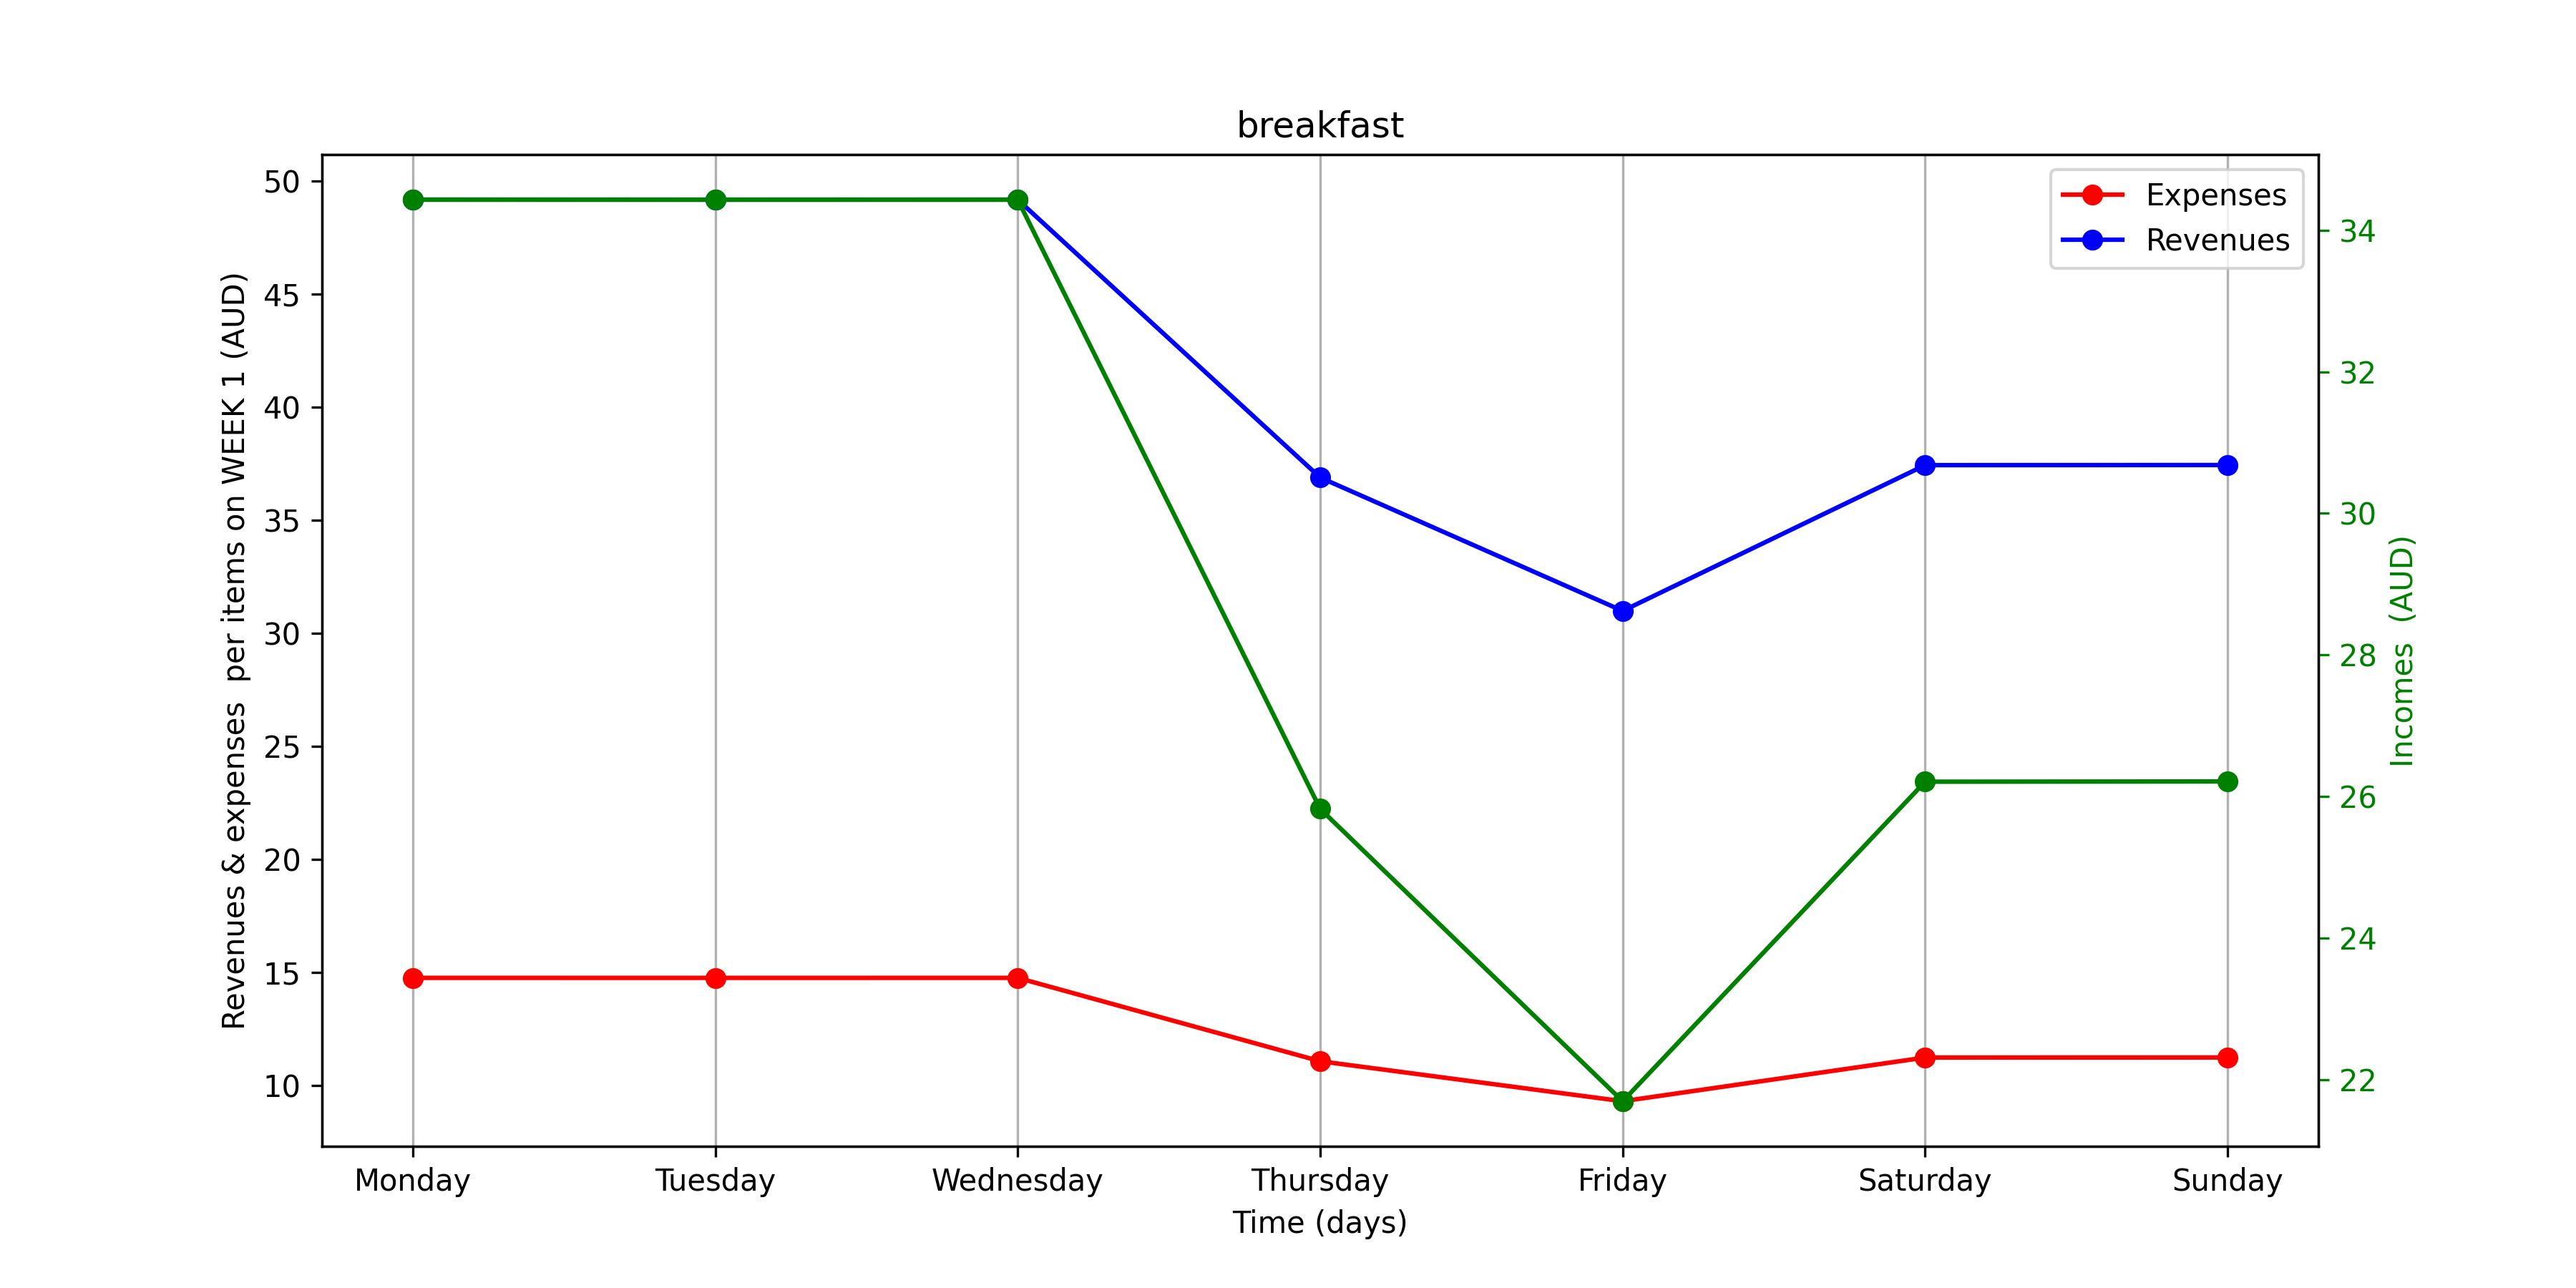
\includegraphics[angle=0, scale=0.5]{graphics/Fig_breakfast.jpg}
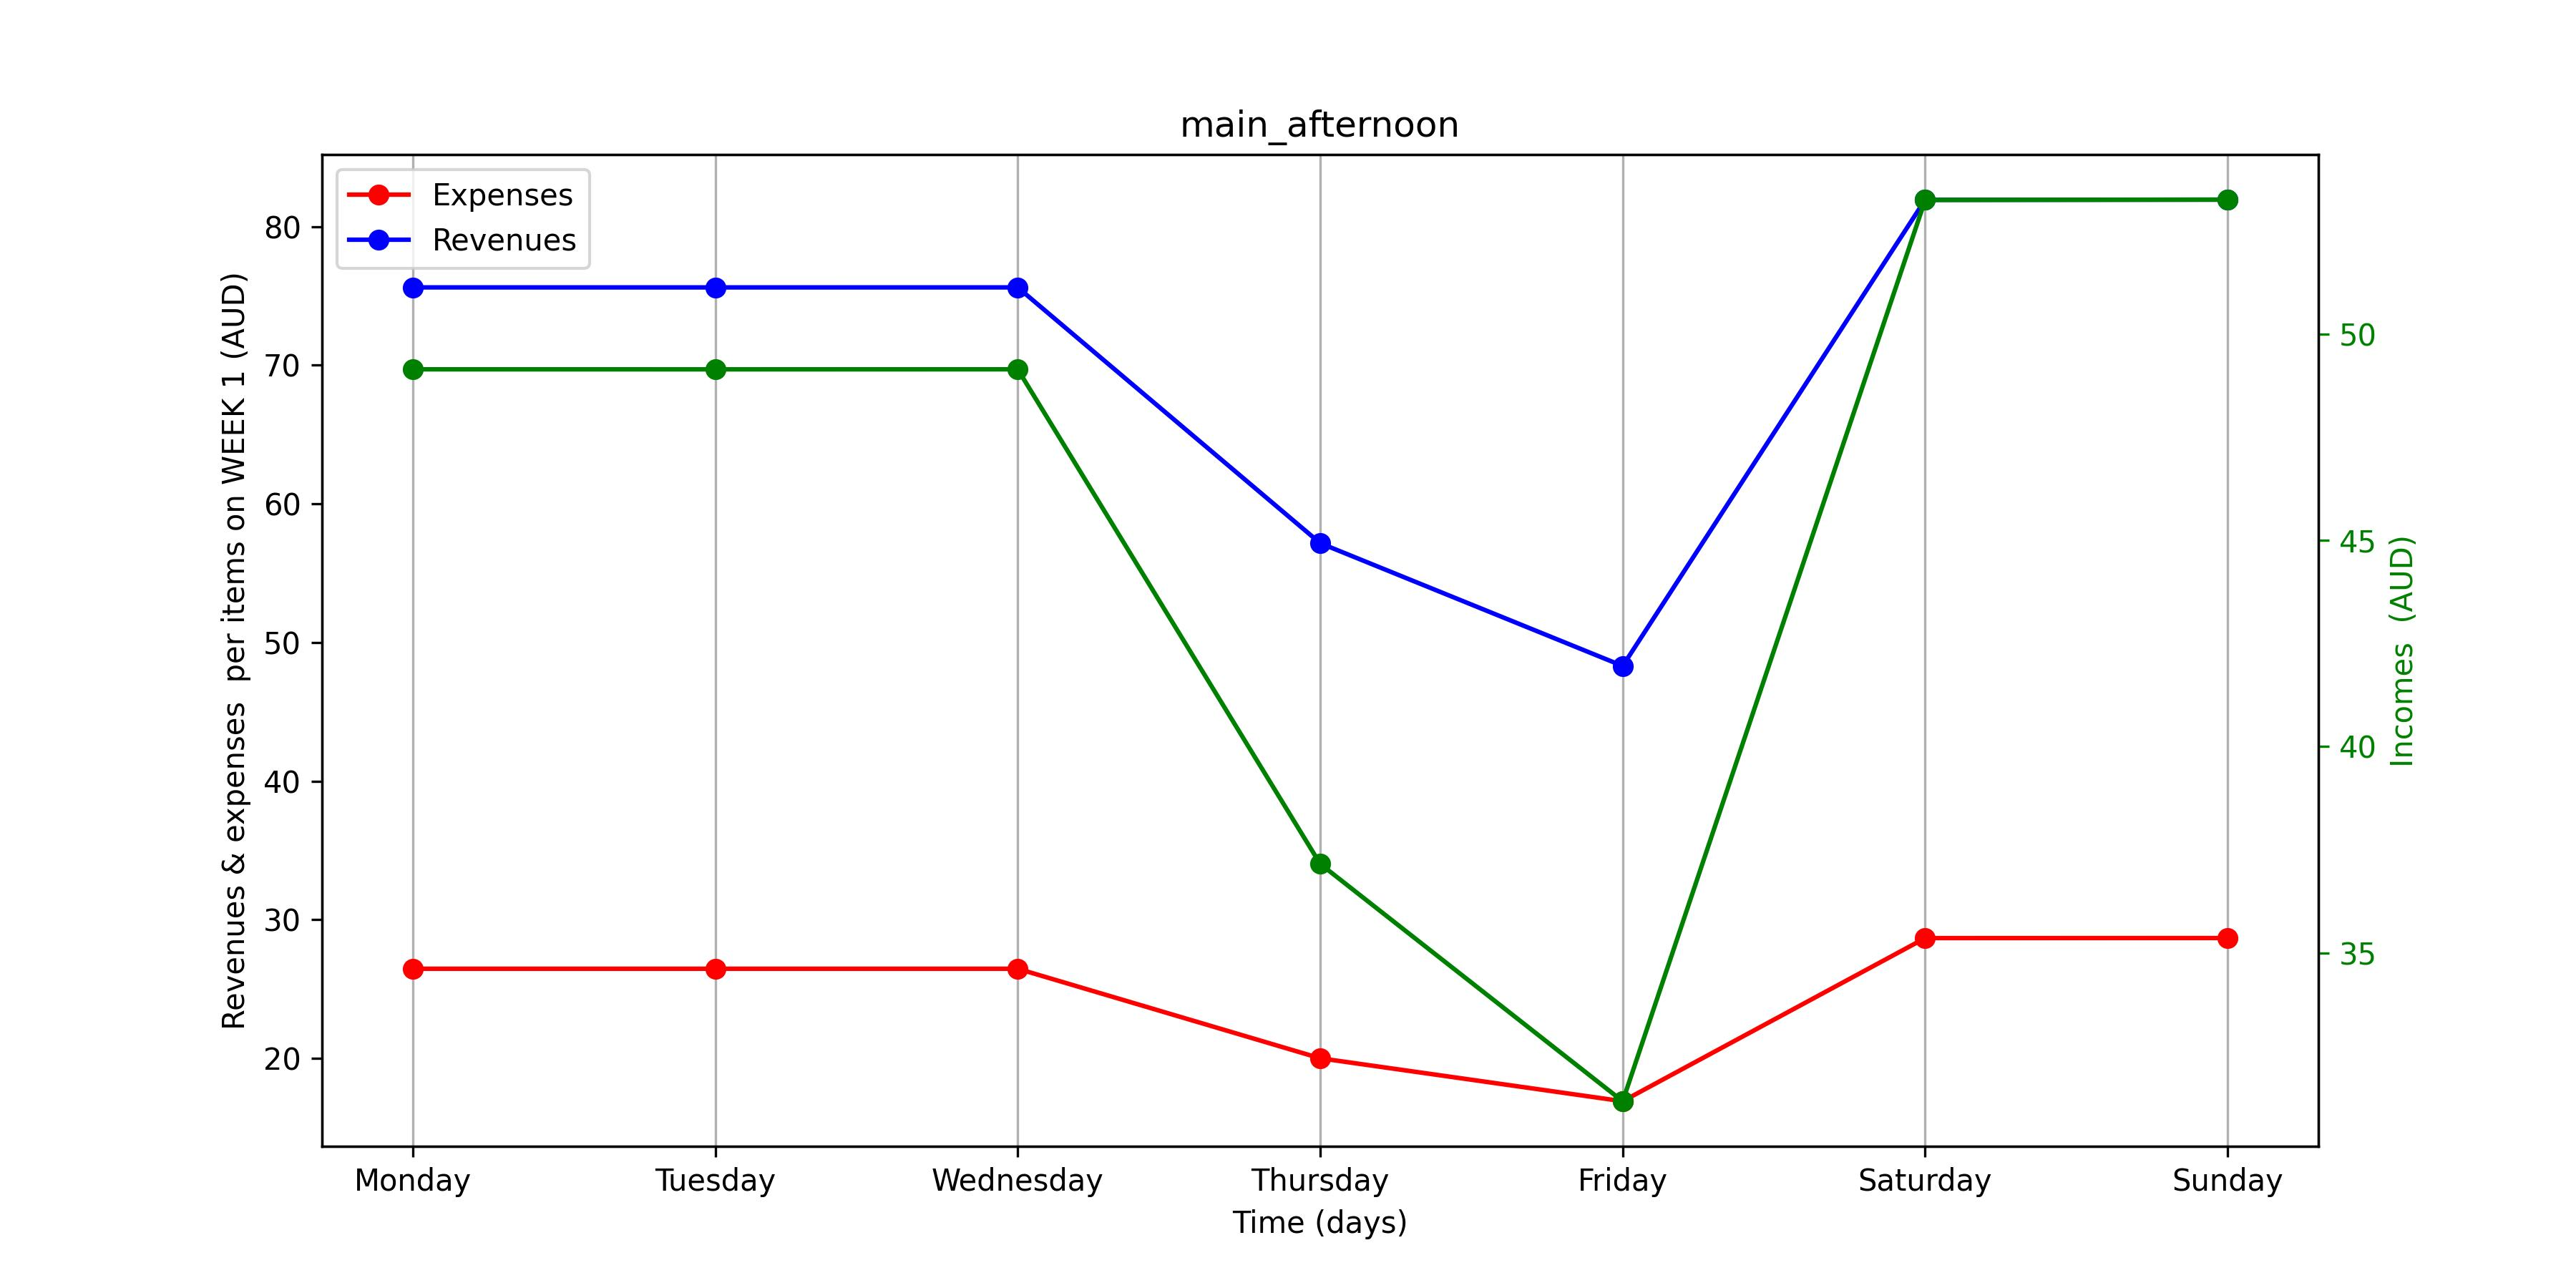
\includegraphics[angle=0, scale=0.5]{graphics/Fig_main_afternoon.jpg}
\caption{(Example of revenue, costs and incomes for breakfasts and main launch as a function of the day of the week and for the first week of January.}
\end{center}
\end{figure}

 \begin{figure}
 \begin{center}
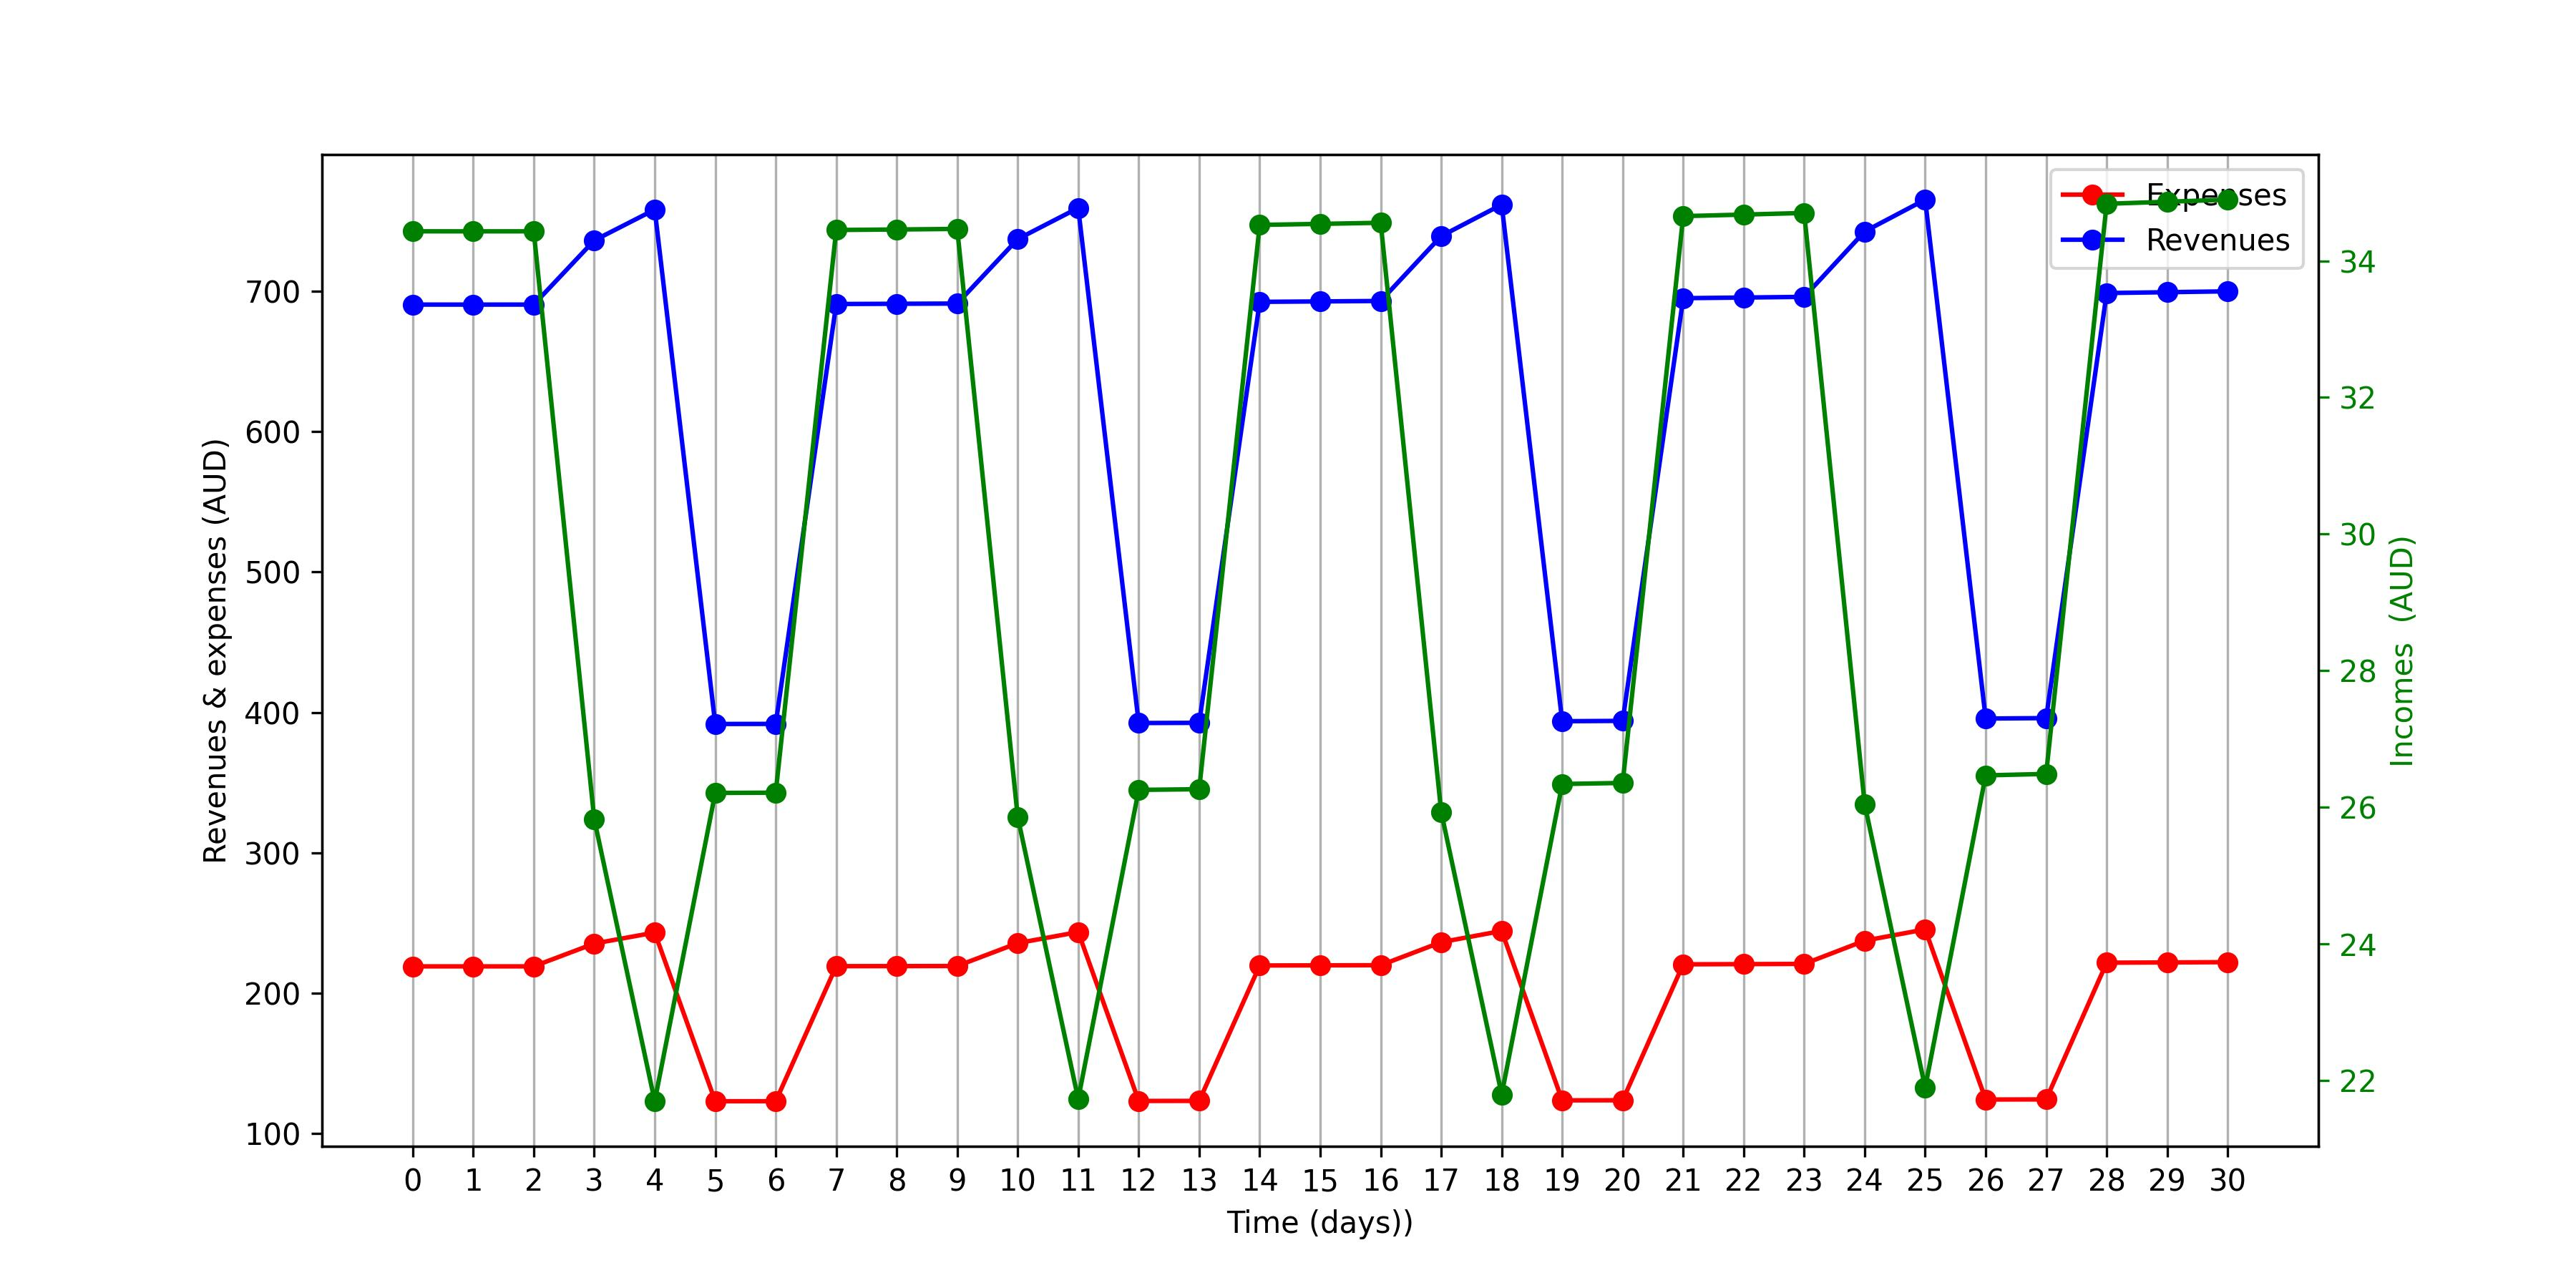
\includegraphics[angle=0, scale=0.5]{graphics/Fig_Jan.jpg}
\caption{(Example of total revenue, costs and incomes as a function of the day of the week and for the first week of Januar.}
\end{center}
\end{figure}

 \begin{figure}
 \begin{center}
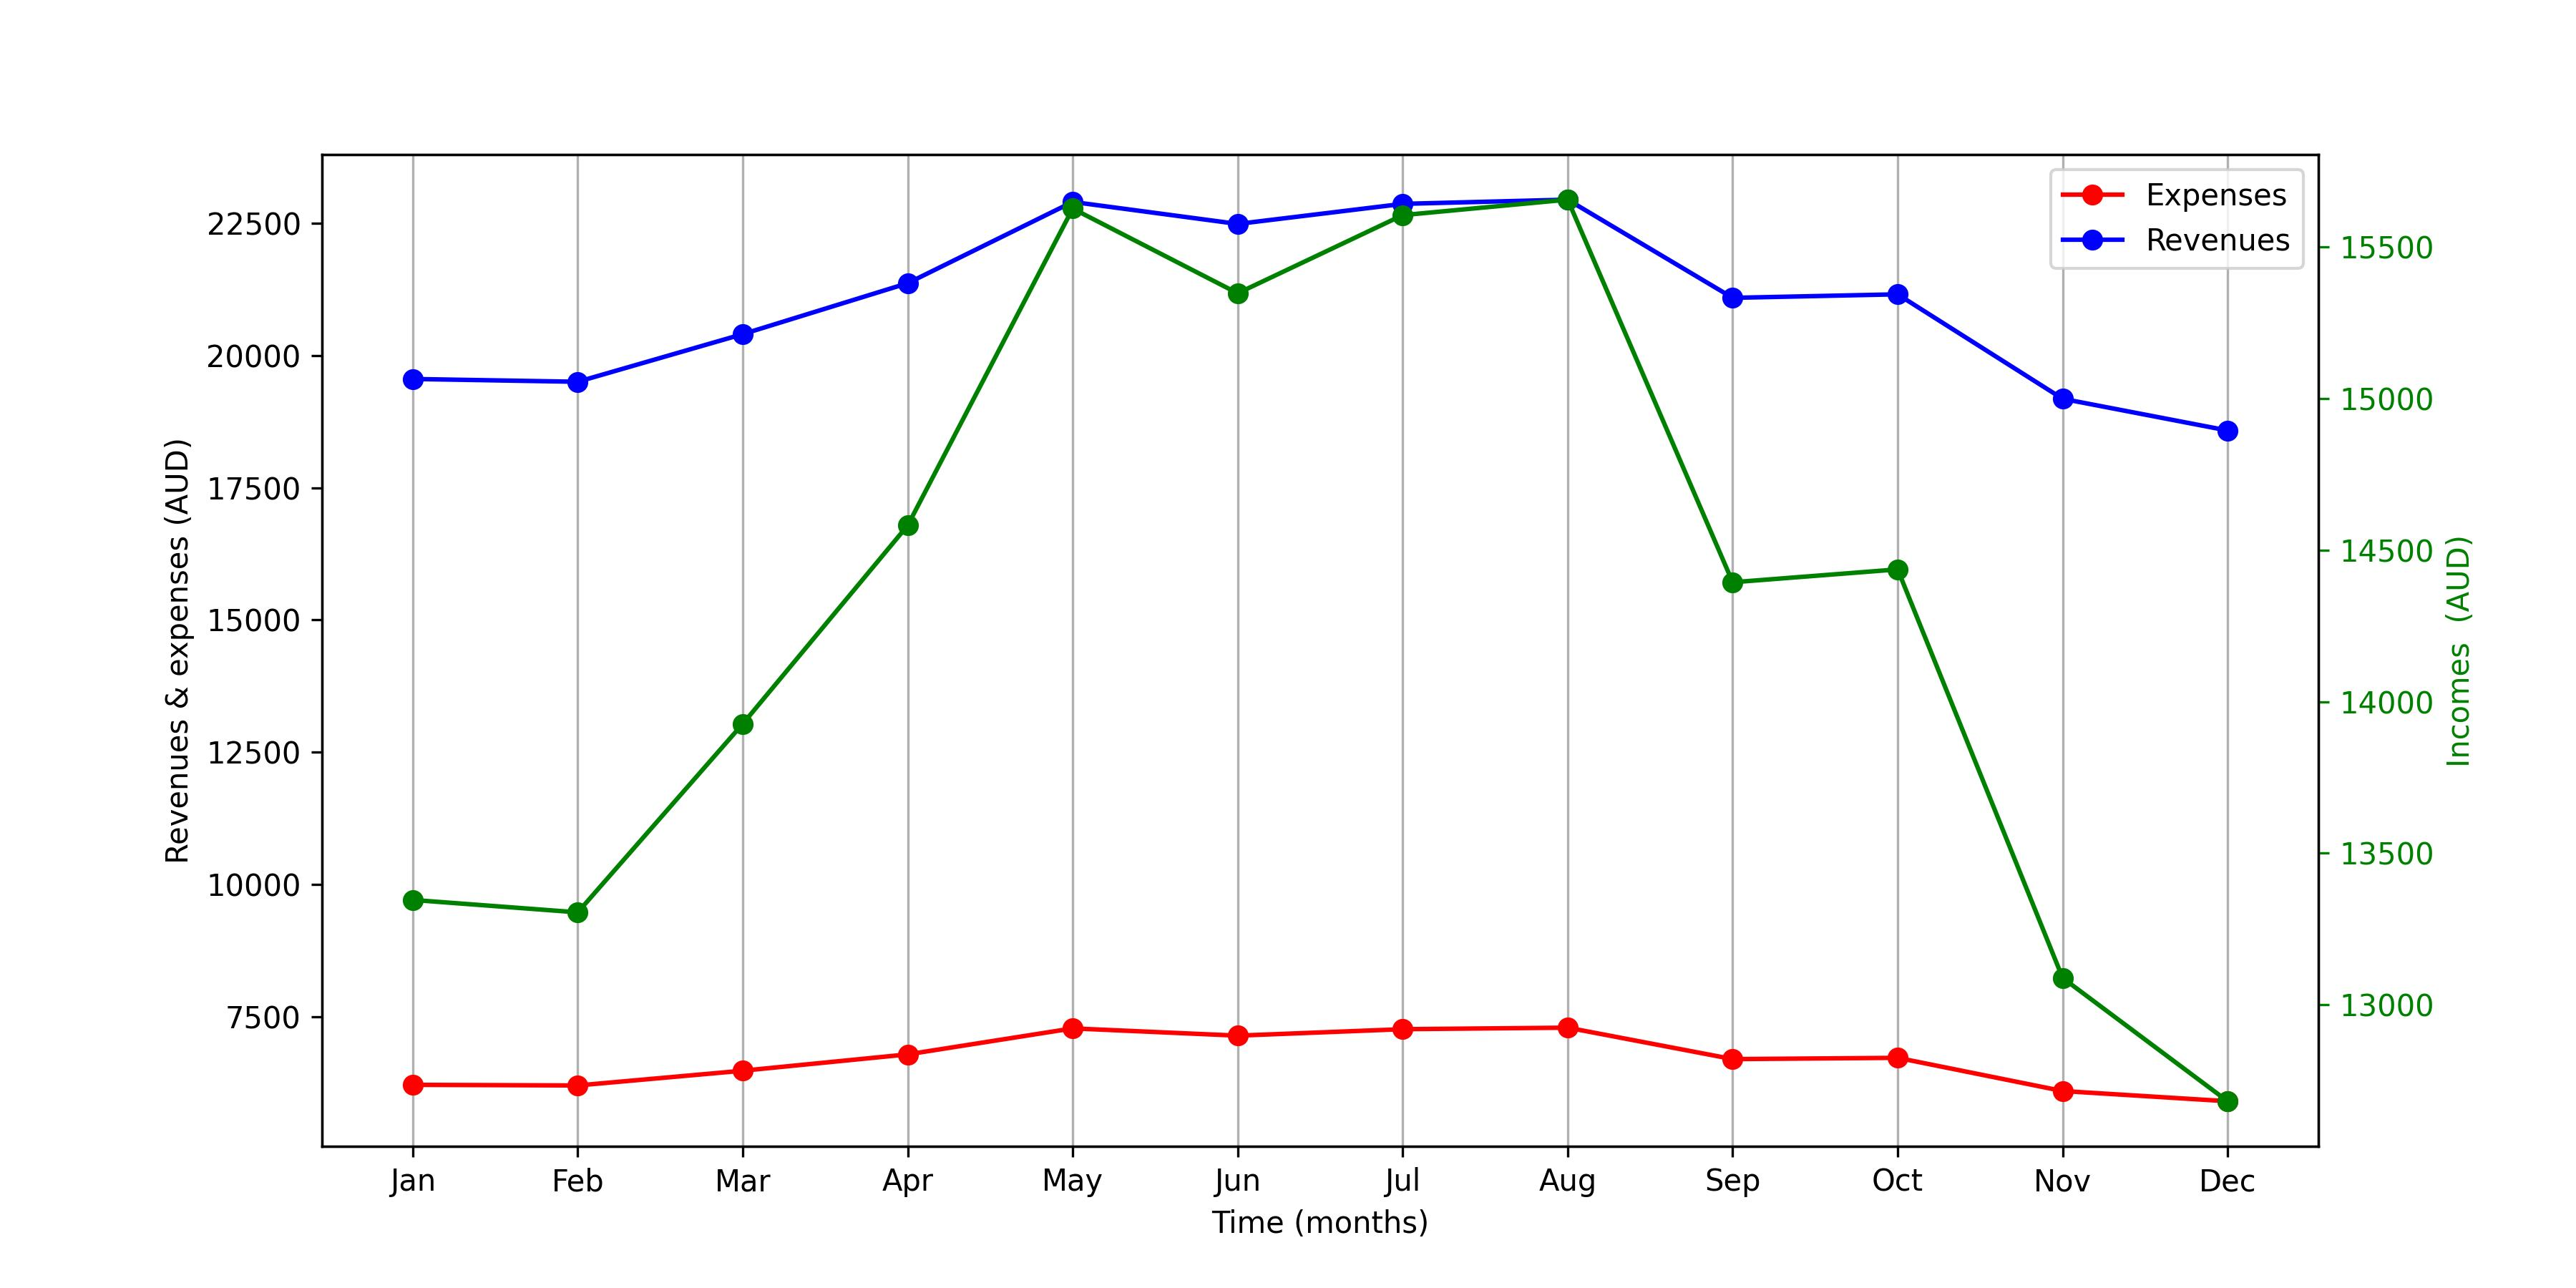
\includegraphics[angle=0, scale=0.5]{graphics/Fig_Year.jpg}
\caption{(Example of monthly revenue, costs and incomes for the study case.}
\end{center}
\end{figure}


%\section{Conclusion} \label{sec:7}

%\bibliographystyle{plain}
%\bibliography{refs}
%\nocite{*}

\end{document}
